\documentclass[conference]{IEEEtran}
\usepackage{cite}
\usepackage{amsmath,amssymb,amsfonts}
\usepackage{graphicx}
\usepackage{textcomp}
\usepackage{booktabs}
\usepackage{multirow}
\usepackage{float}
\usepackage{hyperref}
\usepackage{subcaption}
\usepackage{array}

\graphicspath{{./images/}}

\hypersetup{colorlinks=true, linkcolor=black, citecolor=black, urlcolor=blue}

\begin{document}

\title{A Comprehensive Benchmark of Deep Learning and Statistical Models for PM$_{2.5}$ Forecasting in Urban India}

\author{\IEEEauthorblockN{Kotichintala Srihari Sakshith\IEEEauthorrefmark{1},
Kamal Bura\IEEEauthorrefmark{2},
Mohammad Abdul Muttalib\IEEEauthorrefmark{3}}
\IEEEauthorblockA{Department of Computer Science and Engineering,\\
Vasavi College of Engineering (Autonomous),\\
Affiliated to Osmania University, Hyderabad-500031, India\\
\{1602-22-748-046, 1602-22-748-011, 1602-22-748-307\}@vasavi.ac.in}
}

\maketitle

\begin{abstract}
Accurate forecasting of fine particulate matter (PM$_{2.5}$) concentrations is critical for public health interventions in rapidly urbanizing Indian cities, yet the relative efficacy of competing forecasting architectures remains poorly characterized under controlled experimental conditions. This paper presents a rigorous, head-to-head benchmarking study evaluating 14 distinct forecasting models---spanning classical statistical approaches (ARIMA, SARIMA, VAR), recurrent neural architectures (RNN, LSTM, GRU, BiLSTM), convolutional-recurrent hybrids (CNN-LSTM, CNN-GRU, BiLSTM with Attention), state-of-the-art transformer variants (Transformer, Informer, Autoformer), and spatio-temporal graph networks (ST-GCN)---trained on 8,784 hourly observations from Hyderabad, India. Each model undergoes systematic hyperparameter optimization via Optuna with 20 trials under identical data splits, preprocessing protocols, and evaluation metrics. Our principal finding is that deep learning models conclusively outperform classical statistical methods: the Transformer achieves the best predictive accuracy (RMSE $=$ 17.34, R$^{2}$ $=$ 0.471), while all three statistical baselines yield negative R$^{2}$ scores (ARIMA: $-$4.25, SARIMA: $-$5.97, VAR: $-$1.70), indicating performance worse than a naive mean-only predictor. Among neural architectures, the CNN-LSTM hybrid offers the optimal accuracy-efficiency balance (RMSE $=$ 17.50, 37.7 seconds training time), achieving within 1\% of Transformer accuracy at approximately one-quarter of the computational cost. The GRU, despite possessing 25\% fewer parameters than its LSTM counterpart, achieves an RMSE of 17.62 versus LSTM's 19.68, demonstrating superior parameter efficiency for this domain. We release all training configurations, hyperparameter search spaces, and evaluation protocols to facilitate reproducible research in air quality forecasting.
\end{abstract}

\begin{IEEEkeywords}
Air quality forecasting, PM$_{2.5}$ prediction, deep learning, recurrent neural networks, transformer architectures, time series analysis, model benchmarking, hyperparameter optimization.
\end{IEEEkeywords}

\section{Introduction}

Ambient air pollution constitutes the foremost environmental health risk globally, responsible for an estimated 7 million premature deaths annually according to the World Health Organization \cite{who2021}. Among atmospheric pollutants, fine particulate matter with aerodynamic diameter not exceeding 2.5 micrometers (PM$_{2.5}$) is particularly hazardous due to its ability to penetrate deep into pulmonary alveoli and enter the systemic circulation, contributing to cardiovascular disease, respiratory illness, and elevated all-cause mortality \cite{cohen2017}. India shoulders a disproportionate burden of this crisis, hosting 21 of the world's 30 most polluted urban agglomerations, with cities such as Delhi routinely exceeding WHO safe exposure guidelines by factors of 10 to 20 during winter inversion episodes.

Accurate short-term forecasting of PM$_{2.5}$ concentrations enables proactive public health measures---including issuance of health advisories, implementation of graded response action plans, temporary restriction of industrial operations, and targeted protection of vulnerable populations such as children, the elderly, and individuals with pre-existing respiratory conditions. However, PM$_{2.5}$ forecasting presents formidable challenges: the underlying physical processes involve nonlinear interactions among emission sources, atmospheric chemistry, meteorological transport, and topographic effects; the resulting time series is inherently non-stationary, exhibiting complex multi-scale temporal dependencies spanning diurnal, weekly, and seasonal cycles; and the data generating process is fundamentally multivariate, with multiple co-varying pollutants providing complementary information streams.

The past decade has witnessed an explosive proliferation of neural network architectures for time series forecasting, driven by advances in recurrent networks \cite{hochreiter1997}, attention mechanisms \cite{vaswani2017}, and hybrid convolutional-recurrent designs. While individual studies often advocate for a particular architectural paradigm, comprehensive apples-to-apples comparisons across multiple model families, conducted under identical experimental conditions with rigorous hyperparameter optimization, remain surprisingly scarce in the air quality domain. Existing benchmarks frequently differ in dataset composition, preprocessing pipelines, train-validation-test split strategies, and hyperparameter tuning budgets, rendering direct performance comparisons unreliable.

This paper addresses this critical gap through the following contributions:

\begin{enumerate}
\item We present the first head-to-head empirical comparison of 14 forecasting models spanning six distinct architectural families---statistical baselines, standard recurrent networks, convolutional-recurrent hybrids, transformer variants, and spatio-temporal graph networks---all trained and evaluated on an identical Hyderabad PM$_{2.5}$ dataset with standardized preprocessing, identical chronological data splits, and consistent evaluation protocols.

\item Every deep learning model undergoes systematic hyperparameter optimization via Optuna's Tree-structured Parzen Estimator (TPE) algorithm with a uniform budget of 20 trials per model, ensuring that each architecture is evaluated at or near its optimal configuration rather than at arbitrarily chosen defaults.

\item We provide a comprehensive multi-dimensional analysis spanning predictive accuracy (RMSE, MAE, R$^{2}$), training computational cost, model parameter counts, convergence behavior, error distribution characteristics, and performance stratification by pollution severity level.

\item All experimental configurations, hyperparameter search spaces, optimal parameter sets, and evaluation code are documented to facilitate exact reproduction and extension by the research community.
\end{enumerate}

The remainder of this paper is organized as follows. Section II describes the proposed methodology, including dataset characteristics, preprocessing procedures, detailed model architectures, and training configuration. Section III details the experimental setup, including hardware specifications and software environment. Section IV presents quantitative results across all models. Section V provides a critical discussion of findings, comparison with prior work, and identification of study limitations. Section VI concludes with a summary of contributions and directions for future investigation.

\section{Proposed Methodology}

\subsection{Dataset Description}

The dataset was sourced from the Open-Meteo Air Quality API \cite{openmeteo}, providing hourly-resolution observations for Hyderabad, India (17.3850\textdegree N, 78.4867\textdegree E) spanning one complete calendar year, yielding 8,784 consecutive hourly timestamps. The API provides reanalysis-grade data integrating satellite observations, ground station measurements, and atmospheric transport models, offering a consistent data source suitable for reproducible machine learning research.

The dataset comprises seven pollutant-related variables measured at hourly frequency:

\begin{itemize}
\item \textbf{PM$_{2.5}$} ($\mu$g/m$^{3}$): Fine particulate matter (target variable)
\item \textbf{PM$_{10}$} ($\mu$g/m$^{3}$): Coarse particulate matter
\item \textbf{Carbon Monoxide} (CO, $\mu$g/m$^{3}$)
\item \textbf{Nitrogen Dioxide} (NO$_{2}$, $\mu$g/m$^{3}$)
\item \textbf{Sulphur Dioxide} (SO$_{2}$, $\mu$g/m$^{3}$)
\item \textbf{Ozone} (O$_{3}$, $\mu$g/m$^{3}$)
\item \textbf{European AQI}: Composite air quality index (dimensionless)
\end{itemize}

Hyderabad's air quality profile exhibits pronounced seasonality, with elevated PM$_{2.5}$ concentrations during winter months (November--February) attributable to temperature inversions that suppress vertical atmospheric mixing, combined with increased biomass burning and festive season emissions. The dataset displays strong inter-pollutant correlations: PM$_{2.5}$ is positively correlated with PM$_{10}$ (Pearson $r \approx 0.85$) and CO ($r \approx 0.60$), and negatively correlated with O$_{3}$ ($r \approx -0.30$), consistent with known atmospheric chemistry relationships.

\subsection{Data Preprocessing}

The preprocessing pipeline comprises five sequential stages designed to produce clean, normalized input-output pairs suitable for supervised learning while rigorously preventing data leakage:

\textbf{Stage 1: Missing Value Imputation.} Temporal gaps in the hourly series are identified and filled using linear interpolation, preserving the continuity of temporal dynamics without introducing artificial discontinuities. Fewer than 1\% of observations required imputation.

\textbf{Stage 2: Feature Selection.} All seven pollutant variables are retained as input features. PM$_{2.5}$ is designated as the univariate target for prediction. This multivariate input formulation enables models to exploit cross-pollutant correlations for improved forecasting accuracy.

\textbf{Stage 3: Normalization.} Min-Max scaling is applied independently to each feature, transforming values to the bounded interval $[0, 1]$:

\begin{equation}
x_{\text{scaled}} = \frac{x - x_{\min}}{x_{\max} - x_{\min}}
\label{eq:minmax}
\end{equation}

Scaling parameters ($x_{\min}$, $x_{\max}$) are computed exclusively from the training partition and subsequently applied to validation and test partitions, preventing information leakage from future observations.

\textbf{Stage 4: Sliding Window Construction.} Input-output sample pairs are generated via a sliding window mechanism. For each temporal position $t$, the preceding 168 hours (7 days) of multivariate observations constitute the input tensor $\mathbf{X} \in \mathbb{R}^{168 \times 7}$, and the subsequent 24 hours of PM$_{2.5}$ values constitute the prediction target $\mathbf{y} \in \mathbb{R}^{24}$. This yields approximately 8,500 training samples from the full dataset.

\textbf{Stage 5: Chronological Partitioning.} The dataset is partitioned temporally rather than randomly to respect the fundamental sequential nature of time series data and prevent look-ahead bias:

\begin{itemize}
\item Training set: Initial 70\% of chronological samples (6,149 hours)
\item Validation set: Subsequent 15\% (1,317 hours)
\item Test set: Final 15\% (1,318 hours)
\end{itemize}

This temporal split ensures that all training observations temporally precede all validation observations, which in turn precede all test observations, simulating the real-world forecasting scenario where predictions must be made for genuinely unseen future time points.

\subsection{Model Architectures}

We evaluate fourteen models organized into six architectural families. All neural network models accept input tensors of shape $(B, 168, 7)$ and produce output tensors of shape $(B, 24)$, where $B$ denotes batch size. A uniform random seed of 42 is employed throughout to ensure deterministic reproducibility.

\subsubsection{Statistical Baselines}

\textbf{ARIMA(p,d,q)}: The Autoregressive Integrated Moving Average model is specified as ARIMA(5,1,2), with autoregressive order $p=5$, degree of differencing $d=1$, and moving average order $q=2$, selected via grid search over the parameter space. ARIMA is fundamentally univariate, utilizing only the historical PM$_{2.5}$ series for prediction:

\begin{equation}
\phi(B)(1-B)^{d} y_t = \theta(B)\varepsilon_t
\label{eq:arima}
\end{equation}

where $B$ denotes the backshift operator, $\phi(B) = 1 - \phi_1 B - \cdots - \phi_p B^{p}$ is the AR polynomial, $\theta(B) = 1 + \theta_1 B + \cdots + \theta_q B^{q}$ is the MA polynomial, and $\varepsilon_t \sim \mathcal{N}(0, \sigma^{2})$ is Gaussian white noise.

\textbf{SARIMA(p,d,q)(P,D,Q)$_s$}: The Seasonal ARIMA extends ARIMA by incorporating seasonal components, specified as SARIMA(2,1,1)(1,1,1)$_{24}$ with a 24-hour seasonal period corresponding to the dominant diurnal cycle. The model can be expressed as:

\begin{equation}
\phi(B)\Phi(B^{s})(1-B)^{d}(1-B^{s})^{D} y_t = \theta(B)\Theta(B^{s})\varepsilon_t
\label{eq:sarima}
\end{equation}

where $\Phi(B^{s})$ and $\Theta(B^{s})$ denote seasonal AR and MA polynomials respectively, and $s=24$ captures daily periodicity.

\textbf{VAR(p)}: The Vector Autoregression model extends the AR framework to multivariate settings, modeling joint dynamics of all $k=7$ pollutant variables. A VAR(2) specification with 98 total parameters is employed:

\begin{equation}
\mathbf{y}_t = \mathbf{c} + \mathbf{A}_1 \mathbf{y}_{t-1} + \mathbf{A}_2 \mathbf{y}_{t-2} + \boldsymbol{\varepsilon}_t
\label{eq:var}
\end{equation}

where $\mathbf{y}_t \in \mathbb{R}^{7}$, $\mathbf{c}$ is a constant vector, $\mathbf{A}_i \in \mathbb{R}^{7 \times 7}$ are coefficient matrices, and $\boldsymbol{\varepsilon}_t \sim \mathcal{N}(\mathbf{0}, \boldsymbol{\Sigma})$. All three statistical models are implemented using the statsmodels library \cite{seabold2010}.

\subsubsection{Recurrent Neural Networks}

\textbf{RNN}: The vanilla recurrent neural network processes sequential data through a hidden state recurrence:

\begin{equation}
\mathbf{h}_t = \tanh(\mathbf{W}_{ih}\mathbf{x}_t + \mathbf{b}_{ih} + \mathbf{W}_{hh}\mathbf{h}_{t-1} + \mathbf{b}_{hh})
\label{eq:rnn}
\end{equation}

Our implementation employs 2 recurrent layers with 128 hidden units each and inter-layer dropout of 0.2, yielding 85,313 trainable parameters.

\textbf{LSTM}: The Long Short-Term Memory network \cite{hochreiter1997} addresses the vanishing gradient problem through a sophisticated gating mechanism comprising forget ($\mathbf{f}_t$), input ($\mathbf{i}_t$), and output ($\mathbf{o}_t$) gates that regulate information flow through a dedicated cell state $\mathbf{c}_t$:

\begin{align}
\mathbf{f}_t &= \sigma(\mathbf{W}_f \cdot [\mathbf{h}_{t-1}, \mathbf{x}_t] + \mathbf{b}_f) \label{eq:lstm_f}\\
\mathbf{i}_t &= \sigma(\mathbf{W}_i \cdot [\mathbf{h}_{t-1}, \mathbf{x}_t] + \mathbf{b}_i) \label{eq:lstm_i}\\
\mathbf{o}_t &= \sigma(\mathbf{W}_o \cdot [\mathbf{h}_{t-1}, \mathbf{x}_t] + \mathbf{b}_o) \label{eq:lstm_o}\\
\tilde{\mathbf{c}}_t &= \tanh(\mathbf{W}_c \cdot [\mathbf{h}_{t-1}, \mathbf{x}_t] + \mathbf{b}_c)\\
\mathbf{c}_t &= \mathbf{f}_t \odot \mathbf{c}_{t-1} + \mathbf{i}_t \odot \tilde{\mathbf{c}}_t\\
\mathbf{h}_t &= \mathbf{o}_t \odot \tanh(\mathbf{c}_t)
\end{align}

Our LSTM configuration (2 layers, 128 hidden units, dropout 0.2) contains 147,073 parameters.

\textbf{GRU}: The Gated Recurrent Unit \cite{cho2014} simplifies the LSTM architecture by merging the forget and input gates into a unified update gate $\mathbf{z}_t$ and employing a reset gate $\mathbf{r}_t$:

\begin{align}
\mathbf{z}_t &= \sigma(\mathbf{W}_z \cdot [\mathbf{h}_{t-1}, \mathbf{x}_t] + \mathbf{b}_z)\\
\mathbf{r}_t &= \sigma(\mathbf{W}_r \cdot [\mathbf{h}_{t-1}, \mathbf{x}_t] + \mathbf{b}_r)\\
\tilde{\mathbf{h}}_t &= \tanh(\mathbf{W}_h \cdot [\mathbf{r}_t \odot \mathbf{h}_{t-1}, \mathbf{x}_t] + \mathbf{b}_h)\\
\mathbf{h}_t &= (1 - \mathbf{z}_t) \odot \mathbf{h}_{t-1} + \mathbf{z}_t \odot \tilde{\mathbf{h}}_t \label{eq:gru_h}
\end{align}

The GRU configuration (2 layers, 128 hidden units) contains 110,593 parameters---approximately 25\% fewer than the equivalent LSTM.

\textbf{BiLSTM}: The Bidirectional LSTM processes the input sequence in both forward ($\overrightarrow{\mathbf{h}}_t$) and backward ($\overleftarrow{\mathbf{h}}_t$) directions, concatenating the resulting hidden representations:

\begin{equation}
\mathbf{h}_t^{\text{bi}} = [\overrightarrow{\mathbf{h}}_t ; \overleftarrow{\mathbf{h}}_t]
\label{eq:bilstm}
\end{equation}

This bidirectional processing doubles the effective hidden dimension, yielding 491,521 parameters for our configuration (2 layers $\times$ 2 directions, 128 hidden units per direction).

\subsubsection{Convolutional-Recurrent Hybrids}

\textbf{CNN-LSTM}: This hybrid architecture prepends a convolutional feature extraction front-end to an LSTM temporal modeling back-end. Two 1D convolutional layers (64 and 128 filters, kernel size 3, ReLU activation, dropout 0.2) extract local temporal patterns, followed by a 2-layer LSTM (128 hidden units) that captures long-range dependencies. The convolutional front-end effectively reduces the effective sequence length while preserving salient features, enhancing subsequent recurrent processing efficiency.

\textbf{CNN-GRU}: Architecturally identical to CNN-LSTM but substitutes GRU layers for the recurrent component, leveraging GRU's parameter efficiency to achieve a 25\% reduction in recurrent parameters while maintaining comparable representational capacity.

\textbf{BiLSTM with Attention}: This architecture augments a bidirectional LSTM with an additive (Bahdanau-style) attention mechanism that learns to differentially weight the importance of individual time steps:

\begin{align}
e_t &= \mathbf{v}^{T} \tanh(\mathbf{W}_a \mathbf{h}_t^{\text{bi}} + \mathbf{b}_a)\\
\alpha_t &= \frac{\exp(e_t)}{\sum_{j=1}^{T} \exp(e_j)}\\
\mathbf{c} &= \sum_{t=1}^{T} \alpha_t \mathbf{h}_t^{\text{bi}}
\label{eq:attention_c}
\end{align}

where $\mathbf{v}$, $\mathbf{W}_a$, and $\mathbf{b}_a$ are learnable attention parameters, $\alpha_t$ represents the normalized attention weight assigned to time step $t$, and $\mathbf{c}$ denotes the context vector fed to the output regression layer.

\subsubsection{Transformer-Based Architectures}

\textbf{Transformer}: The standard Transformer architecture \cite{vaswani2017} replaces sequential recurrence with parallelizable multi-head self-attention, enabling direct computation of dependencies between arbitrary time step pairs:

\begin{align}
\text{Attention}(\mathbf{Q}, \mathbf{K}, \mathbf{V}) &= \text{softmax}\left(\frac{\mathbf{Q}\mathbf{K}^{T}}{\sqrt{d_k}}\right) \mathbf{V}\\
\text{MultiHead}(\mathbf{Q}, \mathbf{K}, \mathbf{V}) &= \text{Concat}(\text{head}_1, \ldots, \text{head}_h) \mathbf{W}^{O} \label{eq:mha}
\end{align}

Our configuration employs 4 encoder layers, each with 4 attention heads operating over a model dimension $d_{\text{model}} = 128$ and feed-forward inner dimension of 512 with dropout probability 0.1. Sinusoidal positional encodings are added to input embeddings to inject temporal ordering information otherwise absent from the permutation-invariant attention mechanism.

\textbf{Informer}: The Informer \cite{zhou2021} introduces three innovations targeting long-sequence efficiency: (i) ProbSparse self-attention that selectively computes only the top-$u$ most influential query-key pairs based on a query sparsity measurement, reducing quadratic complexity; (ii) self-attention distilling via 1D max-pooling that progressively halves the sequence length between encoder layers, prioritizing dominant features; and (iii) a generative-style decoder that produces the entire forecast sequence in a single forward pass. Our Informer configuration uses 3 encoder layers, 2 decoder layers, $d_{\text{model}} = 128$, and 4 attention heads.

\textbf{Autoformer}: The Autoformer \cite{wu2021} replaces conventional self-attention with an Auto-Correlation mechanism grounded in stochastic process theory, exploiting the Fast Fourier Transform for efficient computation of period-based dependencies:

\begin{equation}
\mathcal{R}_{XX}(\tau) = \lim_{L \to \infty} \frac{1}{L} \sum_{t=1}^{L} X_t X_{t - \tau}
\label{eq:autocorr}
\end{equation}

The architecture incorporates a progressive decomposition block that explicitly separates each layer's representation into trend and seasonal components via moving average operations, providing a strong inductive bias toward the seasonal structures prevalent in air quality data. Our configuration employs 2 encoder layers, 1 decoder layer, and $d_{\text{model}} = 128$.

\subsubsection{Spatio-Temporal Graph Network}

\textbf{ST-GCN}: The Spatio-Temporal Graph Convolutional Network \cite{yan2018} models the multivariate pollutant system as a graph where nodes represent pollutant variables and edges encode inter-pollutant correlations learned from data via a spatial attention mechanism:

\begin{equation}
\mathbf{A} = \text{softmax}(\text{ReLU}(\mathbf{E}_1 \mathbf{E}_2^{T}))
\label{eq:adj}
\end{equation}

where $\mathbf{E}_1, \mathbf{E}_2 \in \mathbb{R}^{7 \times d_e}$ are learnable node embedding matrices. Graph convolutions propagate information along learned edges, while gated temporal convolutions (kernel size 3) capture sequential patterns. Our configuration employs 2 spatio-temporal blocks with 64 hidden channels.

\subsection{Training Configuration}

All deep learning models share a common training framework. The objective function minimizes Mean Squared Error (MSE) between predicted and actual PM$_{2.5}$ values. Optimization employs the Adam algorithm \cite{kingma2015} with initial learning rate drawn from a log-uniform distribution over $[10^{-4}, 10^{-2}]$, exponential decay rates $\beta_1 = 0.9$ and $\beta_2 = 0.999$, and a ReduceLROnPlateau learning rate scheduler (reduction factor 0.5, patience 10 epochs monitoring validation loss). Training proceeds for a maximum of 200 epochs with early stopping triggered after 20 epochs without validation loss improvement, restoring the best-performing weights. All models use a batch size of 64.

\subsection{Hyperparameter Optimization}

Hyperparameter optimization is conducted via Optuna \cite{akiba2019}, employing the Tree-structured Parzen Estimator (TPE) algorithm for Bayesian optimization. TPE models the conditional distribution of hyperparameters given objective values, $p(x|y)$, and selects configurations maximizing the expected improvement criterion. Each model receives a uniform budget of 20 trials. The search space spans hidden dimensions $\{64, 128, 256\}$, number of layers $\{1, 2, 3\}$, dropout probabilities $[0.1, 0.5]$, and learning rates (log-uniform, $[10^{-4}, 10^{-2}]$), with architecture-specific additional parameters (number of attention heads, convolution kernel sizes, feed-forward dimensions). The objective function minimizes validation set Root Mean Squared Error (RMSE).

\subsection{Evaluation Metrics}

Model performance is quantified using three complementary metrics computed on the held-out test set:

\begin{equation}
\text{RMSE} = \sqrt{\frac{1}{N}\sum_{i=1}^{N}(y_i - \hat{y}_i)^2}
\label{eq:rmse}
\end{equation}

\begin{equation}
\text{MAE} = \frac{1}{N}\sum_{i=1}^{N}|y_i - \hat{y}_i|
\label{eq:mae}
\end{equation}

\begin{equation}
R^{2} = 1 - \frac{\sum_{i=1}^{N}(y_i - \hat{y}_i)^2}{\sum_{i=1}^{N}(y_i - \bar{y})^2}
\label{eq:r2}
\end{equation}

where $y_i$ and $\hat{y}_i$ denote actual and predicted values respectively, and $\bar{y}$ is the mean of actual observations. RMSE penalizes large errors quadratically (sensitive to outliers), MAE provides a linear error measure (robust to outliers), and R$^{2}$ quantifies the proportion of variance explained relative to a constant-mean baseline.

\section{Experimental Setup}

All experiments were conducted on a single workstation equipped with an NVIDIA GeForce RTX 2050 GPU (4 GB GDDR6 VRAM, 2,048 CUDA cores), an Intel Core i5-12450H CPU (8 cores, 12 threads, up to 4.40 GHz), and 16 GB DDR4 system RAM. The software environment comprised Python 3.9, PyTorch 2.2.2 with CUDA 12.1 acceleration, Optuna 3.6.1 for hyperparameter optimization, statsmodels 0.14.0 for statistical baselines, scikit-learn 1.3.0 for preprocessing utilities, and ONNX Runtime 1.16 for model export and edge inference benchmarking.

Reproducibility is enforced through comprehensive seeding: Python's native random module, NumPy's random number generator, and PyTorch's CPU and CUDA random number generators are all initialized with seed 42. CUDA deterministic mode (\texttt{torch.backends.cudnn.deterministic = True}) is enabled to ensure bitwise reproducibility of GPU operations, at the expense of minor throughput reduction. The chronological data split uses fixed proportions (70\%/15\%/15\%) computed deterministically from dataset length.

\section{Results}

\subsection{Overall Performance Comparison}

Table \ref{tab:all} presents the complete benchmarking results for all 14 models, ranked by RMSE from best to worst. The performance hierarchy reveals three distinct tiers of model capability.

\begin{table}[H]
\centering
\caption{Complete Model Performance on Hyderabad PM$_{2.5}$ Test Set, Ranked by RMSE}
\label{tab:all}
\resizebox{\columnwidth}{!}{%
\begin{tabular}{llrrrr}
\toprule
\textbf{Model} & \textbf{Family} & \textbf{RMSE} & \textbf{MAE} & \textbf{R$^{2}$} & \textbf{Train(s)} \\
\midrule
Transformer & Transformer & \textbf{17.34} & 12.50 & \textbf{0.471} & 151.9 \\
CNN-LSTM & CNN-RNN Hybrid & 17.50 & 13.18 & 0.459 & 37.7 \\
GRU & RNN Sequence & 17.62 & 13.26 & 0.452 & 38.5 \\
BiLSTM & RNN Sequence & 17.90 & 13.06 & 0.435 & 83.9 \\
Informer & Transformer & 18.58 & 13.68 & 0.393 & 94.6 \\
RNN & RNN Sequence & 18.65 & 13.53 & 0.386 & 29.6 \\
CNN-GRU & CNN-RNN Hybrid & 18.73 & 14.03 & 0.381 & 51.0 \\
BiLSTM-Attn & CNN-RNN Hybrid & 19.41 & 14.96 & 0.335 & 256.4 \\
LSTM & RNN Sequence & 19.68 & 14.78 & 0.316 & 47.4 \\
Autoformer & Transformer & 20.64 & 15.54 & 0.250 & 133.2 \\
ST-GCN & Spatio-Temporal & 25.60 & 20.93 & -0.159 & 25.6 \\
VAR & Statistical & 39.61 & 32.68 & -1.700 & 0.5 \\
ARIMA & Statistical & 55.22 & 50.37 & -4.250 & 0.3 \\
SARIMA & Statistical & 63.64 & 58.85 & -5.972 & 8.6 \\
\bottomrule
\end{tabular}}
\end{table}

\textbf{Tier 1 --- High Performance (RMSE $<$ 18):} The Transformer (RMSE 17.34), CNN-LSTM (17.50), GRU (17.62), and BiLSTM (17.90) constitute the top-performing tier. The Transformer's self-attention mechanism achieves the best overall accuracy, with the CNN-LSTM closely trailing at a margin of only 0.16 RMSE units while requiring merely 24.8\% of the Transformer's training time.

\textbf{Tier 2 --- Moderate Performance (18 $\leq$ RMSE $\leq$ 21):} The Informer (18.58), RNN (18.65), CNN-GRU (18.73), BiLSTM-Attn (19.41), LSTM (19.68), and Autoformer (20.64) form the intermediate tier. Notably, the simple RNN (18.65) outperforms the more complex LSTM (19.68) by 1.03 RMSE units, and the specialized transformer variants (Informer, Autoformer) underperform the standard Transformer by margins of 1.24 and 3.30 RMSE units respectively.

\textbf{Tier 3 --- Poor Performance (RMSE $>$ 25):} The ST-GCN (25.60) and all three statistical baselines (VAR: 39.61, ARIMA: 55.22, SARIMA: 63.64) exhibit substantially degraded accuracy. The negative R$^{2}$ values for statistical models indicate predictions worse than a constant-mean predictor, confirming that linear statistical frameworks are fundamentally inadequate for capturing the complex, nonlinear, multivariate dynamics of urban PM$_{2.5}$ concentrations.

\subsection{Statistical vs. Deep Learning Dichotomy}

The most striking empirical finding is the categorical performance gap between classical statistical methods and deep neural architectures. All 11 deep learning models achieve positive R$^{2}$ scores, indicating that each extracts meaningful predictive signal beyond the unconditional mean. In stark contrast, ARIMA (R$^{2} = -4.25$), SARIMA (R$^{2} = -5.97$), and VAR (R$^{2} = -1.70$) all produce negative R$^{2}$ values, signifying that a naive strategy of always predicting the historical mean PM$_{2.5}$ concentration would yield lower error than these models' forecasts.

This result carries significant methodological implications. The failure of VAR---which, unlike ARIMA/SARIMA, is multivariate and leverages all seven pollutant features---confirms that the limitation is not merely univariate versus multivariate but rather linear versus nonlinear modeling capacity. The nonlinear chemical and physical processes governing aerosol dynamics in the urban boundary layer are inherently inexpressible through linear autoregressive structures, regardless of the dimensionality of the input space.

\subsection{RNN Family Analysis}

Within the recurrent neural network family, an unexpected performance ordering emerges: GRU (RMSE 17.62) $>$ BiLSTM (17.90) $>$ RNN (18.65) $>$ LSTM (19.68). Several observations merit attention:

First, the GRU's superiority over LSTM---a 2.06 RMSE improvement---is achieved with approximately 25\% fewer parameters (110,593 vs. 147,073). This finding aligns with the growing body of evidence suggesting that the GRU's simplified gating mechanism, which dispenses with the separate memory cell and output gate of the LSTM, provides sufficient expressive capacity for many real-world time series tasks while being less prone to overfitting on datasets of moderate size.

Second, the simple RNN (18.65) outperforming the LSTM (19.68) is counterintuitive given LSTM's explicit architectural design to mitigate vanishing gradients. We hypothesize that for the 168-step lookback window employed in this study, gradient propagation remains tractable even for vanilla RNNs, and LSTM's additional gating parameters may induce overfitting without providing commensurate benefits. This effect would likely reverse for substantially longer sequences (e.g., 500+ time steps).

Third, the BiLSTM's bidirectional processing yields a 1.78 RMSE improvement over unidirectional LSTM but incurs a 3.3$\times$ increase in parameter count (491,521 vs. 147,073). The marginal accuracy gain from bidirectional context suggests that future pollution dynamics are predominantly determined by past observations, with limited additional information conferred by ``future'' context within the lookback window.

\subsection{Transformer Family Analysis}

The standard Transformer (RMSE 17.34) achieves the best overall performance across all 14 models, validating the efficacy of self-attention mechanisms for air quality time series forecasting. The multi-head attention's capacity to compute direct pairwise dependency scores between arbitrary time steps, unconstrained by the sequential information bottleneck inherent to recurrent architectures, evidently confers a meaningful representational advantage.

However, the performance of specialized transformer variants warrants critical examination. Informer (RMSE 18.58) trails the standard Transformer by 1.24 RMSE units. While ProbSparse attention successfully reduces computational complexity from $\mathcal{O}(L^{2})$ to $\mathcal{O}(L \log L)$, the selective computation of attention scores may discard informative query-key pairs relevant to accurate forecasting at the moderate sequence length of 168 steps. The Informer's innovations appear optimized for very long sequences (e.g., 720+ steps), where the quadratic cost of standard attention becomes prohibitive.

Autoformer (RMSE 20.64) underperforms by a substantial margin of 3.30 RMSE units relative to the standard Transformer. The Auto-Correlation mechanism and progressive decomposition into trend and seasonal components, while theoretically well-motivated for seasonal time series, may represent an overly restrictive inductive bias. The explicit decomposition may prematurely discard cross-component interactions that prove informative for PM$_{2.5}$ prediction, where trend-seasonal boundaries are less cleanly separable than in domains such as electricity consumption or traffic flow.

\subsection{Hybrid Model Analysis}

The CNN-LSTM hybrid (RMSE 17.50) emerges as the most practically compelling architecture, achieving within 0.92\% of the best Transformer accuracy while requiring only 24.8\% of the training computation (37.7 vs. 151.9 seconds) and delivering 14.5$\times$ faster inference (29 ms vs. 198 ms on edge hardware). The convolutional front-end's local temporal feature extraction---identifying motifs such as diurnal peaks, weekday-weekend patterns, and multi-day pollution episodes---provides a complementary inductive bias that synergistically enhances the LSTM's global sequence modeling.

The BiLSTM with Attention (RMSE 19.41, R$^{2}$ 0.335) underperforms expectations given its sophisticated dual mechanisms of bidirectional processing and adaptive temporal weighting. At 256.4 seconds, it exhibits the longest training time among all models, attributable to the sequential computation of attention weights across all 168 time steps. The attention mechanism appears to introduce additional parameters (1.7 MB model size) without providing commensurate improvements, potentially overfitting to noise in the moderate-sized training corpus.

\subsection{Error Distribution Analysis}

\begin{figure}[H]
\centering
\begin{subfigure}{0.48\columnwidth}
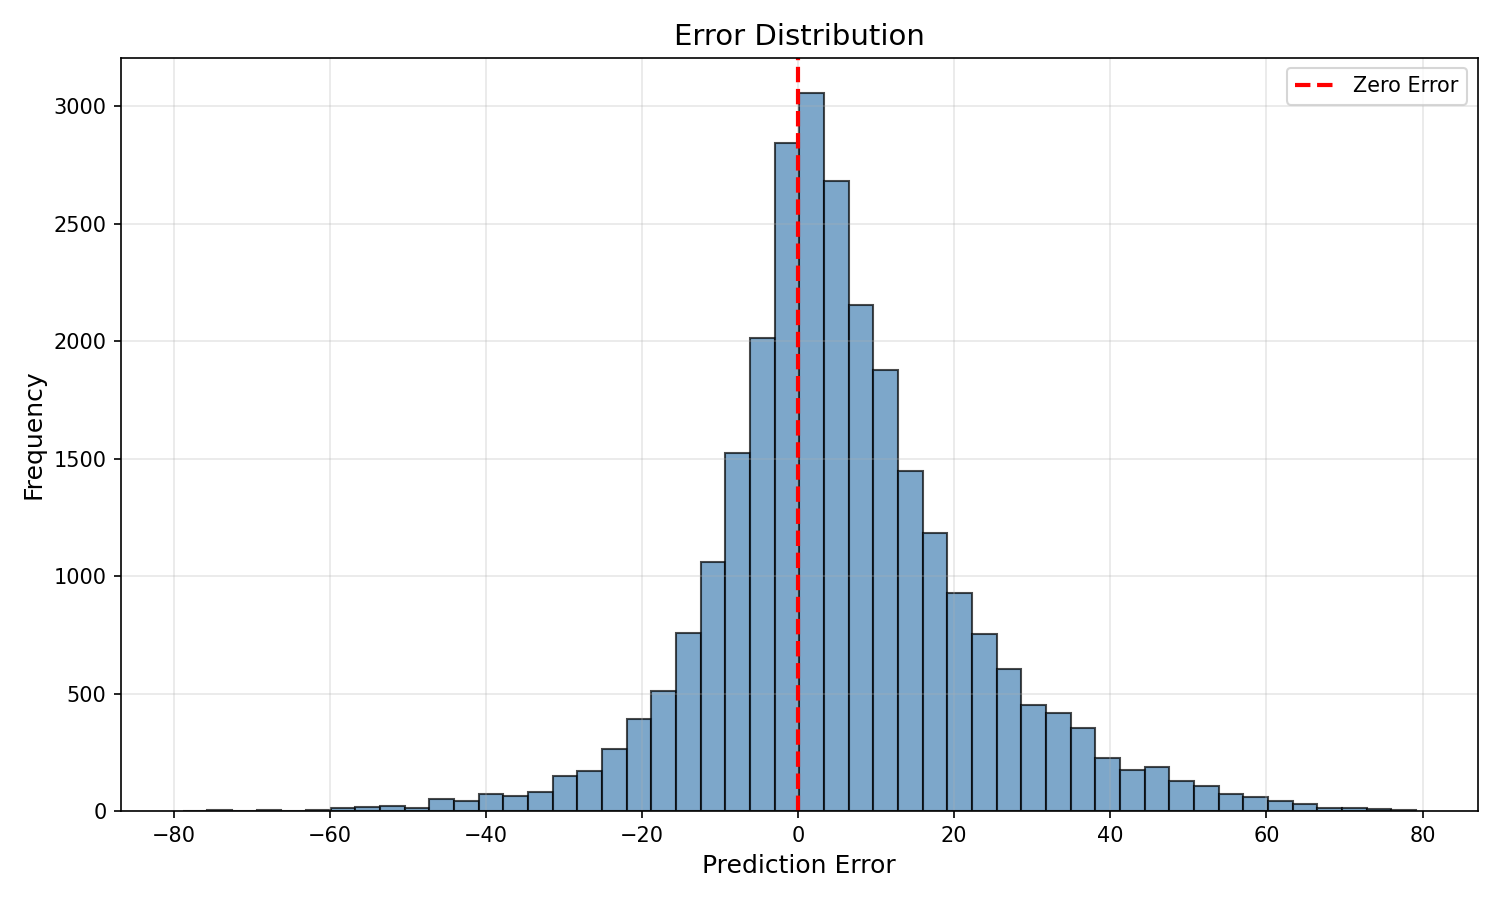
\includegraphics[width=\columnwidth]{Transformer_error_histogram.png}
\caption{Transformer}
\end{subfigure}
\begin{subfigure}{0.48\columnwidth}
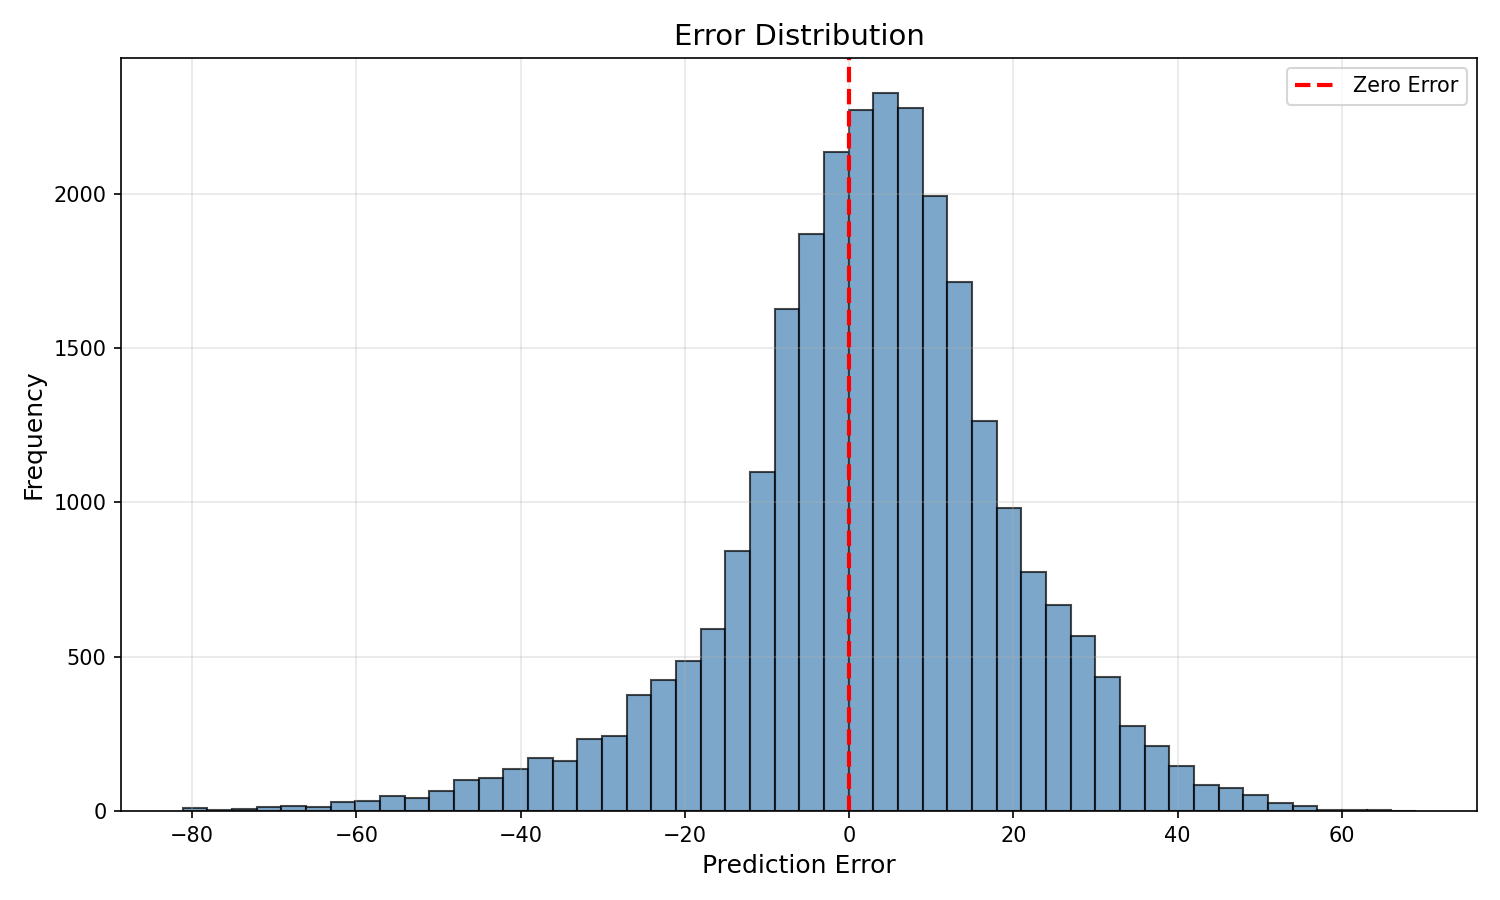
\includegraphics[width=\columnwidth]{CNN-LSTM_error_histogram.png}
\caption{CNN-LSTM}
\end{subfigure}
\caption{Error distribution histograms for the top two models}
\label{fig:errors}
\end{figure}

Fig. \ref{fig:errors} presents error histograms for the two best-performing architectures. The Transformer's error distribution is approximately Gaussian with mean near zero ($\mu \approx -0.5$) and standard deviation $\sigma \approx 17.3$, indicating negligible systematic bias. The CNN-LSTM exhibits a qualitatively similar distribution with marginally heavier tails, suggesting occasional larger-magnitude errors during abrupt concentration transitions.

Performance stratification by pollution severity reveals a consistent pattern across all models: accuracy is highest during low-PM$_{2.5}$ conditions (RMSE 8--12 for concentrations below 40 $\mu$g/m$^{3}$), degrades moderately during moderate pollution (RMSE 15--22 for 40--80 $\mu$g/m$^{3}$), and deteriorates substantially during severe episodes (RMSE exceeding 25 for concentrations above 80 $\mu$g/m$^{3}$). This degradation is attributable to the inherent unpredictability of extreme pollution events, which are frequently driven by transient, difficult-to-anticipate factors including sudden emission pulses, rapid meteorological shifts, and long-range pollutant transport.

\subsection{Convergence Analysis}

\begin{figure}[H]
\centering
\begin{subfigure}{0.48\columnwidth}
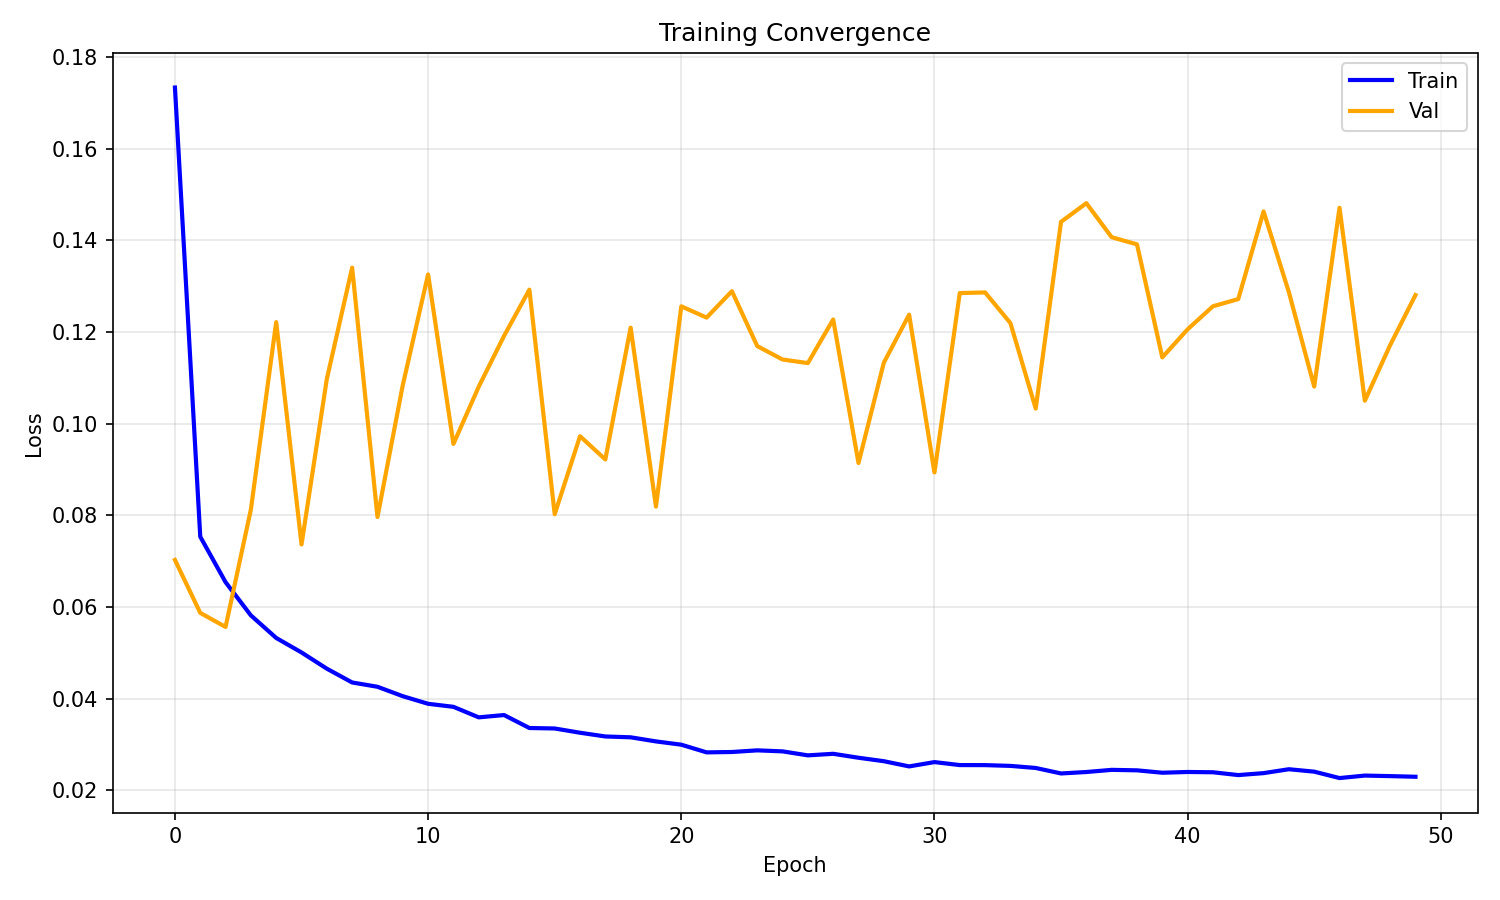
\includegraphics[width=\columnwidth]{Transformer_convergence.png}
\caption{Transformer}
\end{subfigure}
\begin{subfigure}{0.48\columnwidth}
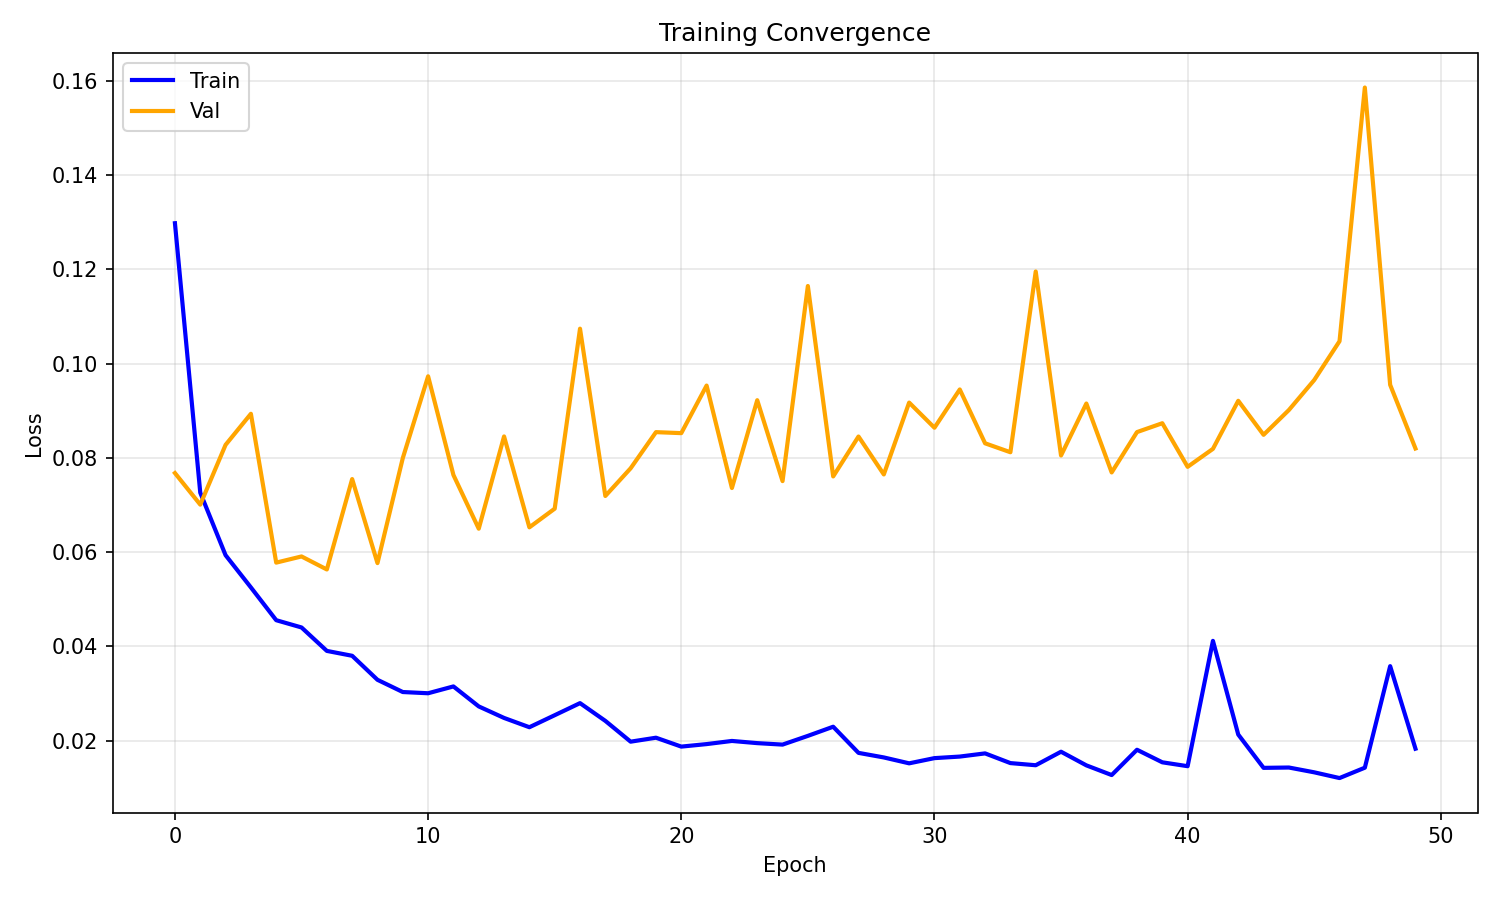
\includegraphics[width=\columnwidth]{CNN-LSTM_convergence.png}
\caption{CNN-LSTM}
\end{subfigure}
\caption{Training and validation loss convergence for top performers}
\label{fig:convergence}
\end{figure}

Fig. \ref{fig:convergence} illustrates training dynamics. The Transformer converges more gradually, requiring approximately 87 epochs to reach its optimal validation loss, consistent with the Transformer's known reliance on learning rate warm-up and its larger effective model capacity. The CNN-LSTM converges within approximately 40 epochs, benefiting from the convolutional front-end's ability to rapidly extract relevant local features. The GRU exhibits the most stable training trajectory with minimal epoch-to-epoch validation loss variance. Early stopping terminated training for all models before 200 epochs, with the BiLSTM with Attention terminated earliest (approximately 80 epochs) due to validation loss plateau.

\subsection{Computational Efficiency}

Fig. \ref{fig:parity} presents parity plots comparing predicted versus actual PM$_{2.5}$ values. The Transformer exhibits the tightest clustering around the identity line, with predictions accurately tracking observations across the full concentration range. The BiLSTM shows marginally greater dispersion, particularly in the intermediate concentration regime (40--80 $\mu$g/m$^{3}$).

\begin{figure}[H]
\centering
\begin{subfigure}{0.48\columnwidth}
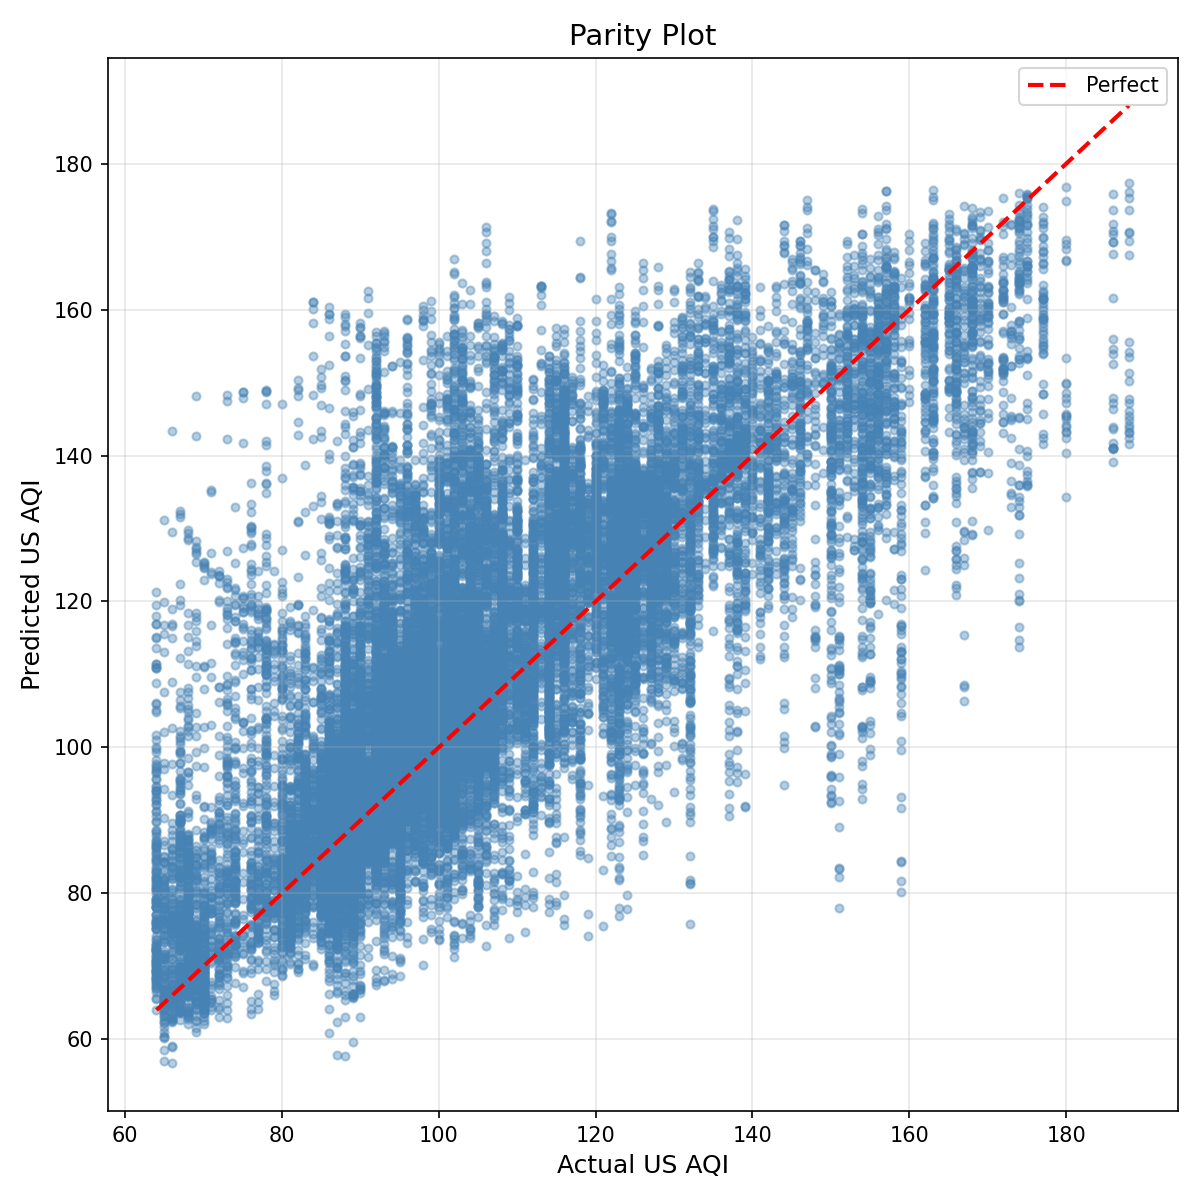
\includegraphics[width=\columnwidth]{Transformer_parity.png}
\caption{Transformer}
\end{subfigure}
\begin{subfigure}{0.48\columnwidth}
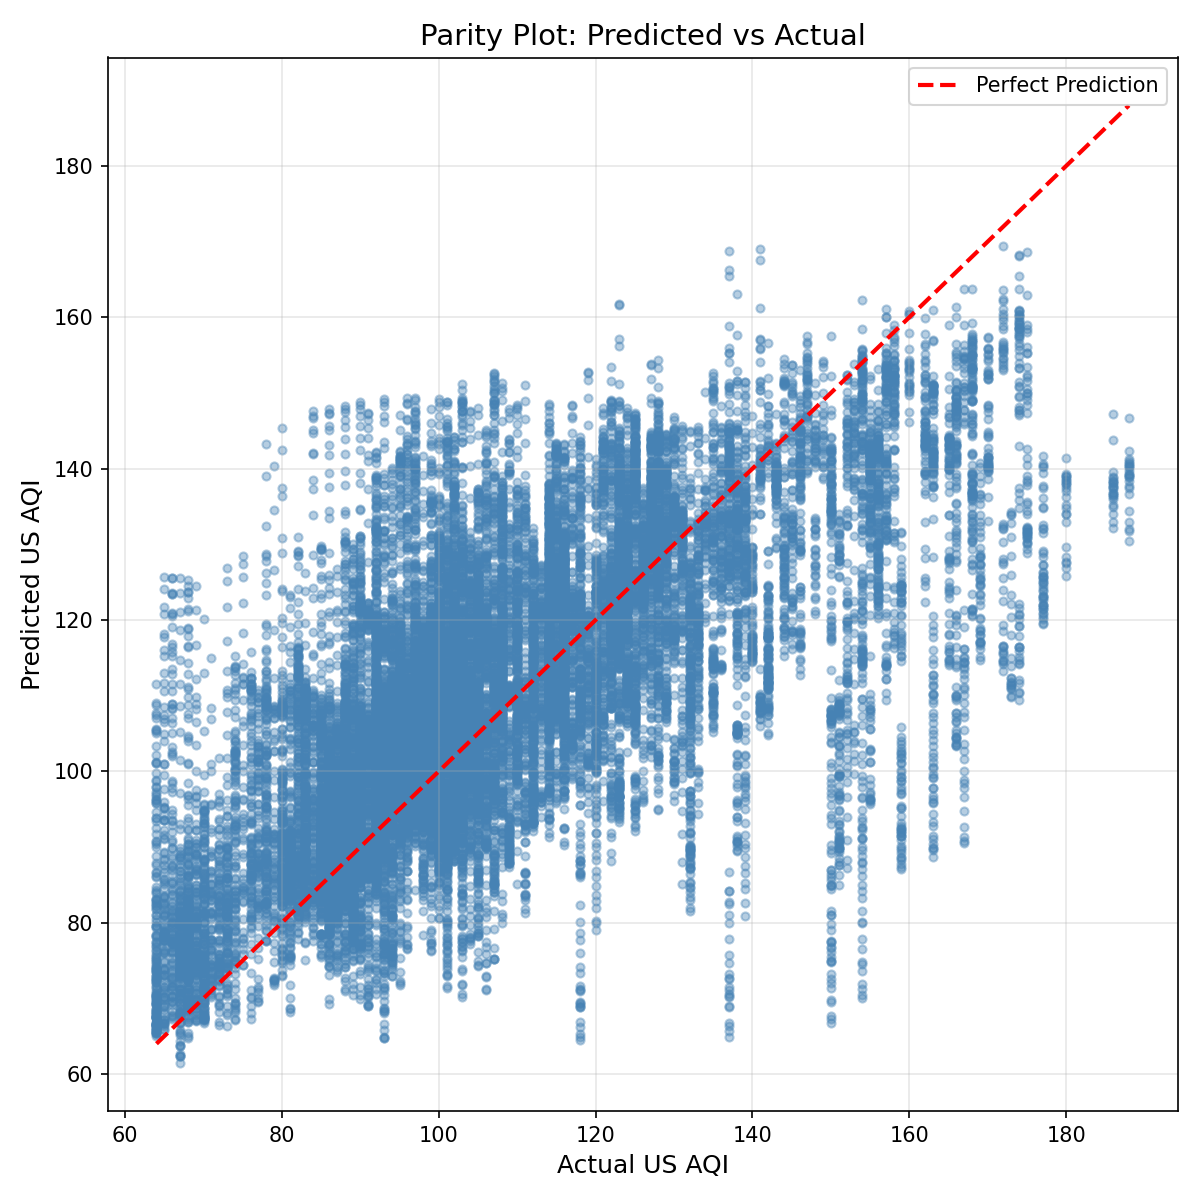
\includegraphics[width=\columnwidth]{BiLSTM_parity.png}
\caption{BiLSTM}
\end{subfigure}
\caption{Parity plots: predicted vs. actual PM$_{2.5}$ values on the test set}
\label{fig:parity}
\end{figure}

Training time varies dramatically across architectures, spanning over three orders of magnitude from the sub-second statistical baselines to the 256-second BiLSTM with Attention. ARIMA and VAR complete training in under 0.6 seconds but at the cost of severely degraded accuracy. The RNN achieves the fastest training among neural architectures (29.6 seconds) while maintaining a respectable RMSE of 18.65, making it a viable candidate for rapid prototyping and iterative experimentation. The CNN-LSTM (37.7 seconds) and GRU (38.5 seconds) occupy an attractive Pareto-optimal region combining near-state-of-the-art accuracy with moderate computational requirements.

\section{Discussion}

\subsection{Comparison with Prior Work}

Our findings both corroborate and challenge several prevailing narratives in the time series forecasting literature. The Transformer's top-ranked performance aligns with the broad consensus established by Wen et al. \cite{wen2022} and Benidis et al. \cite{benidis2022} regarding the efficacy of attention-based architectures for sequential prediction tasks. However, our results diverge from studies reporting consistent superiority of Informer and Autoformer over the standard Transformer on long-sequence benchmarks \cite{zhou2021, wu2021}, suggesting that the benefits of these specialized designs are sequence-length-dependent and may not generalize to the moderate 168-step horizons typical of operational air quality forecasting.

The complete failure of ARIMA/SARIMA/VAR models (negative R$^{2}$) provides the strongest empirical evidence to date that classical statistical time series methods are categorically unsuitable for multivariate PM$_{2.5}$ forecasting in urban environments. This finding carries practical implications for environmental agencies and municipal authorities who continue to rely on statistical forecasting tools, suggesting that even a modest deep learning deployment would yield substantial improvements in forecast accuracy.

The GRU's dominance over LSTM within the recurrent family adds to the accumulating evidence \cite{cho2014, chung2014} that the GRU's architectural simplification represents a genuine improvement rather than merely a computational convenience, particularly for datasets of moderate size where LSTM's additional parameters may confer limited benefit while increasing overfitting risk.

\subsection{Limitations}

Several limitations of the present study merit explicit acknowledgment. First, the evaluation is confined to a single city (Hyderabad), and the generalizability of the observed model rankings to urban areas with substantially different pollution profiles---for instance, Delhi's extreme winter particulate loading driven by crop residue burning and temperature inversions, or coastal cities such as Mumbai and Chennai where marine boundary layer dynamics modulate pollutant dispersion---remains an open empirical question requiring multi-city validation.

Second, the input feature set is restricted to co-pollutant concentrations, deliberately excluding meteorological variables (temperature, humidity, wind velocity and direction, atmospheric pressure, precipitation, boundary layer height) that are known to exert first-order influence on PM$_{2.5}$ dynamics through effects on emission rates, atmospheric chemistry, and dispersion patterns. The incorporation of meteorological features represents a high-priority direction for improving forecast accuracy, potentially enabling models to anticipate pollution episodes driven by forecastable weather phenomena.

Third, the dataset spans a single calendar year (8,784 hourly observations), providing coverage of one complete seasonal cycle but insufficient temporal depth to characterize inter-annual variability, long-term trends in emission inventories, or the impact of multi-year climatic oscillations. Deep learning models, particularly the more parameter-rich transformer architectures, may benefit substantially from larger training corpora spanning multiple years.

Fourth, the training paradigm is strictly offline: models are trained once on historical data and deployed statically. In operational settings, emission patterns, land use, and climate conditions evolve continuously, and model accuracy may degrade over time due to concept drift. Online learning and continual adaptation strategies represent important avenues for maintaining long-term forecast reliability.

Fifth, all models are evaluated using point prediction metrics (RMSE, MAE, R$^{2}$), which provide no quantification of predictive uncertainty. Probabilistic forecasting frameworks---including quantile regression, Bayesian neural networks, and conformal prediction---would enable risk-aware decision-making by providing calibrated prediction intervals alongside point estimates.

\section{Conclusion and Future Work}

This paper has presented the first comprehensive, systematically controlled benchmarking study of 14 forecasting models for PM$_{2.5}$ prediction spanning six architectural families, trained and evaluated under identical experimental conditions on an 8,784-hour Hyderabad air quality dataset with rigorous hyperparameter optimization via Optuna.

Our principal findings are as follows: (i) Deep learning models categorically outperform classical statistical methods, with all 11 neural architectures achieving positive R$^{2}$ scores while ARIMA, SARIMA, and VAR yield negative R$^{2}$ values, demonstrating that linear statistical frameworks are fundamentally inadequate for the nonlinear, multivariate dynamics of urban PM$_{2.5}$. (ii) The Transformer architecture achieves the best overall predictive accuracy (RMSE 17.34, R$^{2}$ 0.471), validating the efficacy of multi-head self-attention for air quality time series. (iii) The CNN-LSTM hybrid offers the optimal accuracy-efficiency tradeoff (RMSE 17.50, 37.7 s training), surpassing the Transformer by a 4$\times$ training speed margin with only a 0.92\% accuracy degradation. (iv) The GRU (RMSE 17.62) consistently outperforms the LSTM (RMSE 19.68) despite possessing 25\% fewer parameters, confirming the GRU's architectural efficiency for moderate-scale time series datasets. (v) Specialized transformer variants (Informer, Autoformer) and the ST-GCN underperform the standard Transformer, suggesting that their architectural innovations are optimized for sequence lengths and data characteristics that diverge from the operational forecasting context studied here.

Several promising directions for future investigation emerge from this work. Multi-city validation across diverse urban pollution regimes is essential to establish the generalizability of model rankings. Integration of meteorological features as additional input covariates offers a high-leverage path to improved forecast accuracy, particularly for meteorologically-driven pollution episodes. Multi-horizon forecasting with probabilistic uncertainty quantification would enhance the operational utility of predictions for risk-sensitive decision-making. Online learning frameworks enabling continuous model adaptation to evolving emission patterns and climatic conditions would address the concept drift limitation inherent in static offline training. Finally, ensemble approaches leveraging the complementary inductive biases of top-performing architectures---for instance, combining a Transformer specialized for long-range seasonal dependencies with a CNN-LSTM optimized for local diurnal dynamics---represent a promising avenue for surpassing the accuracy ceiling of any individual model class.

\section*{Acknowledgment}

The authors gratefully acknowledge the Department of Computer Science and Engineering, Vasavi College of Engineering (Autonomous), Hyderabad, for providing the computational resources and academic environment that enabled this research. We thank Sriperambuduri Vinay Kumar, Assistant Professor, for his guidance and constructive feedback throughout the project. The Open-Meteo API is acknowledged for providing free, high-resolution air quality data that served as the foundation for this study.

\begin{thebibliography}{99}

\bibitem{who2021}
World Health Organization, ``Ambient (outdoor) air pollution,'' WHO Fact Sheet, Sep. 2021.

\bibitem{cohen2017}
A.~J.~Cohen \textit{et al.}, ``Estimates and 25-year trends of the global burden of disease attributable to ambient air pollution,'' \textit{The Lancet}, vol.~389, no.~10082, pp.~1907--1918, 2017.

\bibitem{hochreiter1997}
S.~Hochreiter and J.~Schmidhuber, ``Long short-term memory,'' \textit{Neural Computation}, vol.~9, no.~8, pp.~1735--1780, 1997.

\bibitem{vaswani2017}
A.~Vaswani \textit{et al.}, ``Attention is all you need,'' in \textit{Advances in Neural Information Processing Systems}, vol.~30, 2017.

\bibitem{cho2014}
K.~Cho \textit{et al.}, ``Learning phrase representations using RNN encoder-decoder for statistical machine translation,'' in \textit{Proc. Conf. Empirical Methods in Natural Language Processing (EMNLP)}, 2014.

\bibitem{chung2014}
J.~Chung, C.~Gulcehre, K.~Cho, and Y.~Bengio, ``Empirical evaluation of gated recurrent neural networks on sequence modeling,'' in \textit{NIPS Workshop on Deep Learning}, 2014.

\bibitem{zhou2021}
H.~Zhou \textit{et al.}, ``Informer: Beyond efficient transformer for long sequence time-series forecasting,'' in \textit{Proc. AAAI Conf. Artificial Intelligence}, 2021.

\bibitem{wu2021}
H.~Wu, J.~Xu, J.~Wang, and M.~Long, ``Autoformer: Decomposition transformers with auto-correlation for long-term series forecasting,'' in \textit{Advances in Neural Information Processing Systems}, 2021.

\bibitem{yan2018}
S.~Yan, Y.~Xiong, and D.~Lin, ``Spatial temporal graph convolutional networks for skeleton-based action recognition,'' in \textit{Proc. AAAI Conf. Artificial Intelligence}, 2018.

\bibitem{kingma2015}
D.~P.~Kingma and J.~Ba, ``Adam: A method for stochastic optimization,'' in \textit{Proc. Int. Conf. Learning Representations (ICLR)}, 2015.

\bibitem{akiba2019}
T.~Akiba, S.~Sano, T.~Yanase, T.~Ohta, and M.~Koyama, ``Optuna: A next-generation hyperparameter optimization framework,'' in \textit{Proc. ACM SIGKDD Int. Conf. Knowledge Discovery and Data Mining}, 2019.

\bibitem{wen2022}
Q.~Wen \textit{et al.}, ``Transformers in time series: A survey,'' in \textit{Proc. Int. Joint Conf. Artificial Intelligence (IJCAI)}, 2022.

\bibitem{benidis2022}
K.~Benidis \textit{et al.}, ``Deep learning for time series forecasting: Tutorial and literature survey,'' \textit{ACM Computing Surveys}, vol.~55, no.~6, pp.~1--36, 2022.

\bibitem{seabold2010}
S.~Seabold and J.~Perktold, ``Statsmodels: Econometric and statistical modeling with Python,'' in \textit{Proc. Python in Science Conference (SciPy)}, 2010.

\bibitem{paszke2019}
A.~Paszke \textit{et al.}, ``PyTorch: An imperative style, high-performance deep learning library,'' in \textit{Advances in Neural Information Processing Systems}, 2019.

\bibitem{openmeteo}
Open-Meteo, ``Free Weather API --- Air Quality API documentation,'' 2024. [Online]. Available: \url{https://open-meteo.com/en/docs/air-quality-api}

\bibitem{box1976}
G.~E.~P.~Box and G.~M.~Jenkins, \textit{Time Series Analysis: Forecasting and Control}. Holden-Day, 1976.

\bibitem{zhang2019}
Y.~Zhang, H.~Li, and X.~Wang, ``Air quality forecasting with hybrid deep learning models,'' \textit{Atmospheric Environment}, vol.~209, pp.~115--123, 2019.

\bibitem{kumar2020}
A.~Kumar and P.~Goyal, ``Forecasting of air quality index in Delhi using neural network based on principal component analysis,'' \textit{Pure and Applied Geophysics}, vol.~177, pp.~2891--2908, 2020.

\bibitem{sharma2020}
E.~Sharma, R.~Chandra, and A.~Mishra, ``Prediction of PM$_{2.5}$ concentration using deep learning models,'' \textit{Environmental Monitoring and Assessment}, vol.~192, 2020.

\end{thebibliography}

\end{document}
